\section{Behavioral, Interaction, and User-Interface Design}
\label{sec:behavioral-ui}

\safesubsection{Activity Diagrams}
\label{subsec:activity-diagrams}
System workflows, guard conditions, concurrency checks, and exception branches are modeled using five monochrome UML 2.5 swimlane Activity Diagrams synchronized with the delivered V2.2 platform:
\begin{itemize}
  \item \textbf{Shared EV Rental Lifecycle (\Cref{fig:act-rental}):} Traces hub search, atomic overlap \& battery checks ($\ge 20\%$), \texttt{PENDING} creation, Operator approval (\texttt{CONFIRMED}) vs.\ rejection (\texttt{OPERATOR\_\allowbreak REJECTED}), Student optical QR unlock (\texttt{ACTIVE}) vs.\ cancellation/expiry, and capacity-verified hub return (\texttt{COMPLETED}).
  \item \textbf{Parking \& Multi-Charger Scheduling (\Cref{fig:act-charging}):} Models Zone C customer bay booking and \texttt{AUTO} multi-charger port locking where multiple students receive distinct free ports concurrently until hub capacity saturates into the \texttt{QUEUED} priority waitlist.
  \item \textbf{Incident Isolation \& Recovery (\Cref{fig:act-incident}):} Enforces mandatory affected-unit selection, immediate \texttt{OUT\_\allowbreak OF\_\allowbreak SERVICE} isolation, staff assignment (\texttt{IN\_\allowbreak PROGRESS}), and repair-verified restoration.
  \item \textbf{Two-Phase Redistribution \& Priority Queue (\Cref{fig:act-dispatch}):} Illustrates Phase A source-slot vacation and Phase B destination-slot binding (excluding private EVs), alongside 2-table priority re-ranking and charger swaps.
  \item \textbf{What-If Simulation (\Cref{fig:act-sim}):} Depicts read-only snapshot cloning into RAM, 1-minute discrete evolution, impact scoring (\texttt{I1..I8}), and live-state revalidation prior to applying confirmed actions.
\end{itemize}

\begin{figure}[H]
  \centering
  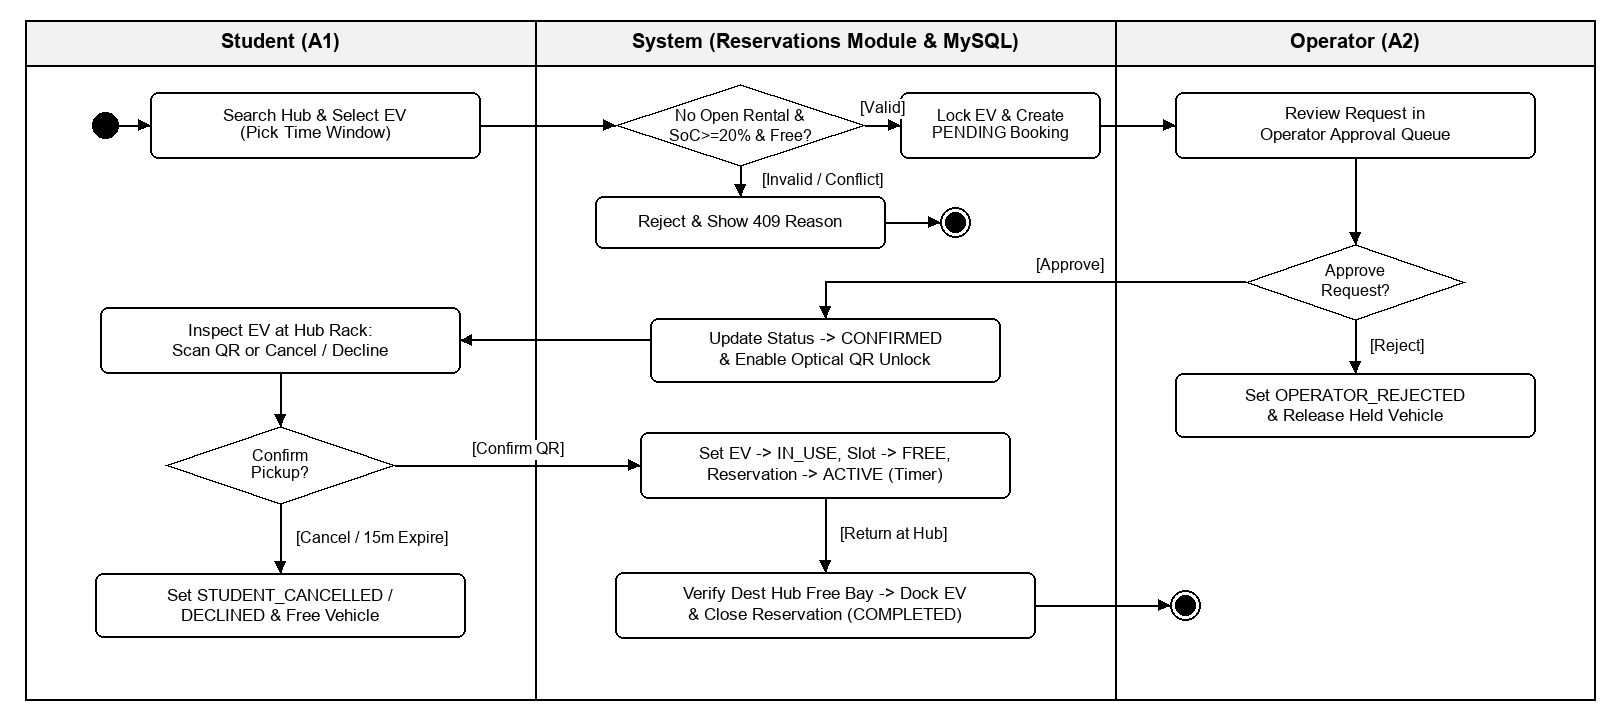
\includegraphics[width=0.92\linewidth]{graphics/diagrams/fig3_1_act_rental.png}
  \caption{Activity Diagram --- 5-Stage Shared EV Reservation, Approval, QR Pickup \& Return}
  \label{fig:act-rental}
\end{figure}

\begin{figure}[H]
  \centering
  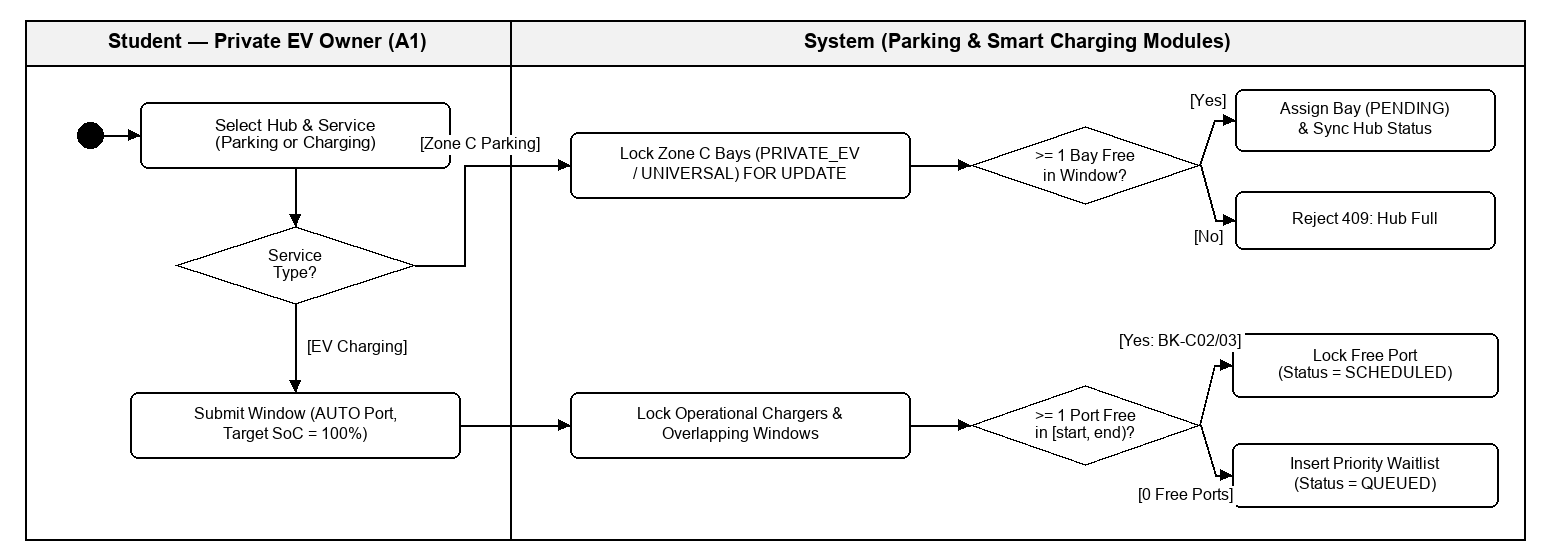
\includegraphics[width=0.90\linewidth]{graphics/diagrams/fig3_2_act_parking_charging.png}
  \caption{Activity Diagram --- Zone C Parking Reservation \& Multi-Charger \texttt{AUTO} Scheduling}
  \label{fig:act-charging}
\end{figure}

\begin{figure}[H]
  \centering
  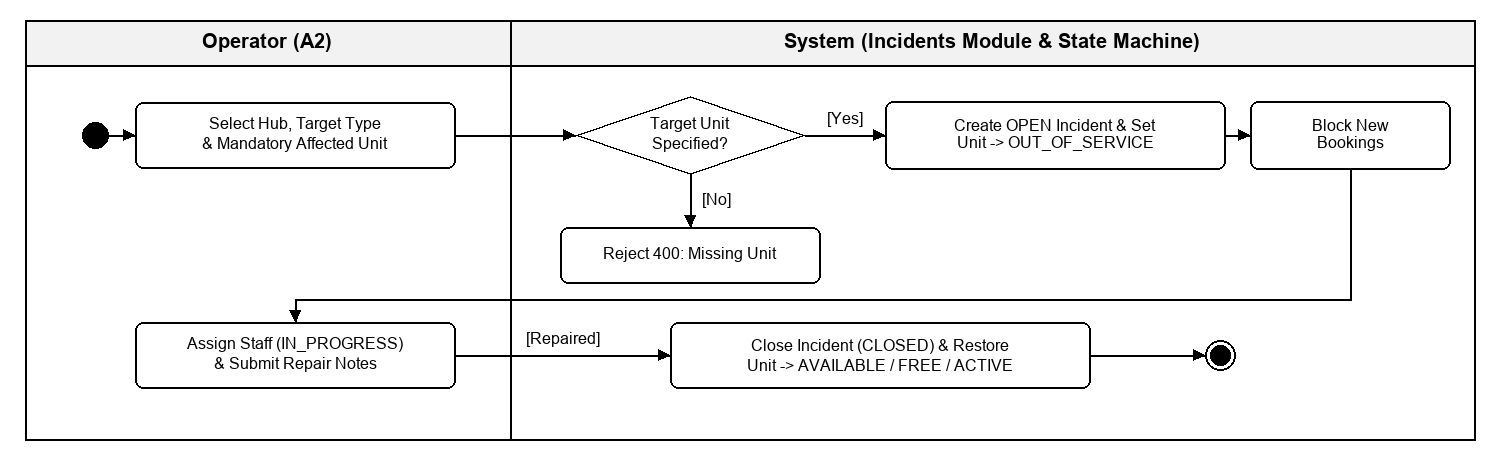
\includegraphics[width=0.90\linewidth]{graphics/diagrams/fig3_3_act_incident.png}
  \caption{Activity Diagram --- Mandatory-Target Incident Isolation \& Repair Resolution}
  \label{fig:act-incident}
\end{figure}

\begin{figure}[H]
  \centering
  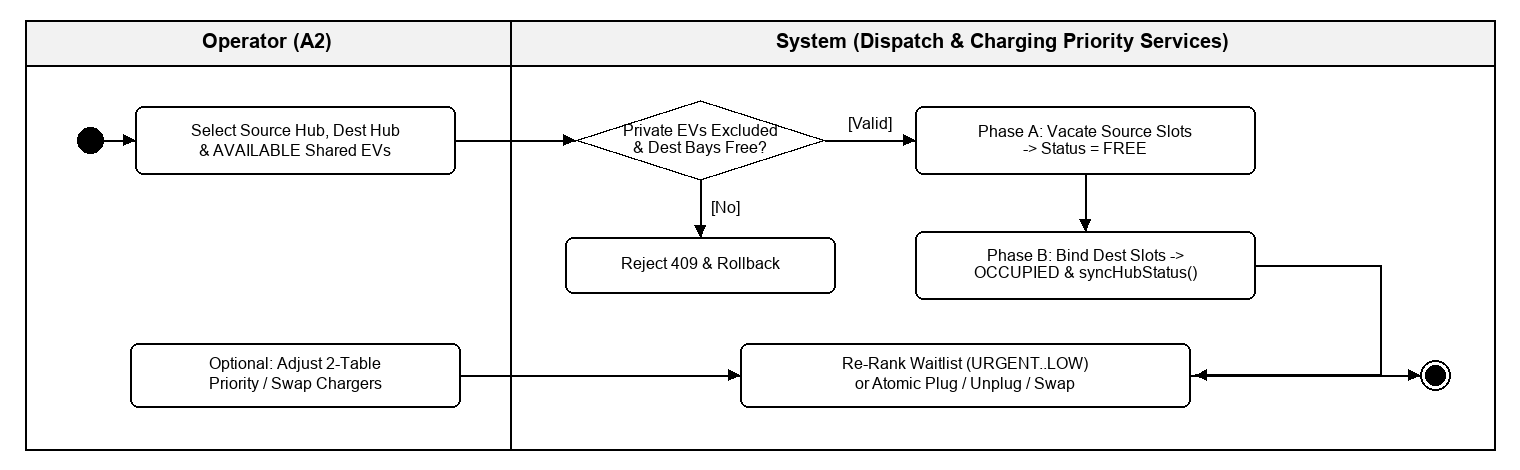
\includegraphics[width=0.90\linewidth]{graphics/diagrams/fig3_4_act_dispatch_priority.png}
  \caption{Activity Diagram --- Two-Phase Slot-to-Slot Vehicle Redistribution \& Charging Priority}
  \label{fig:act-dispatch}
\end{figure}

\begin{figure}[H]
  \centering
  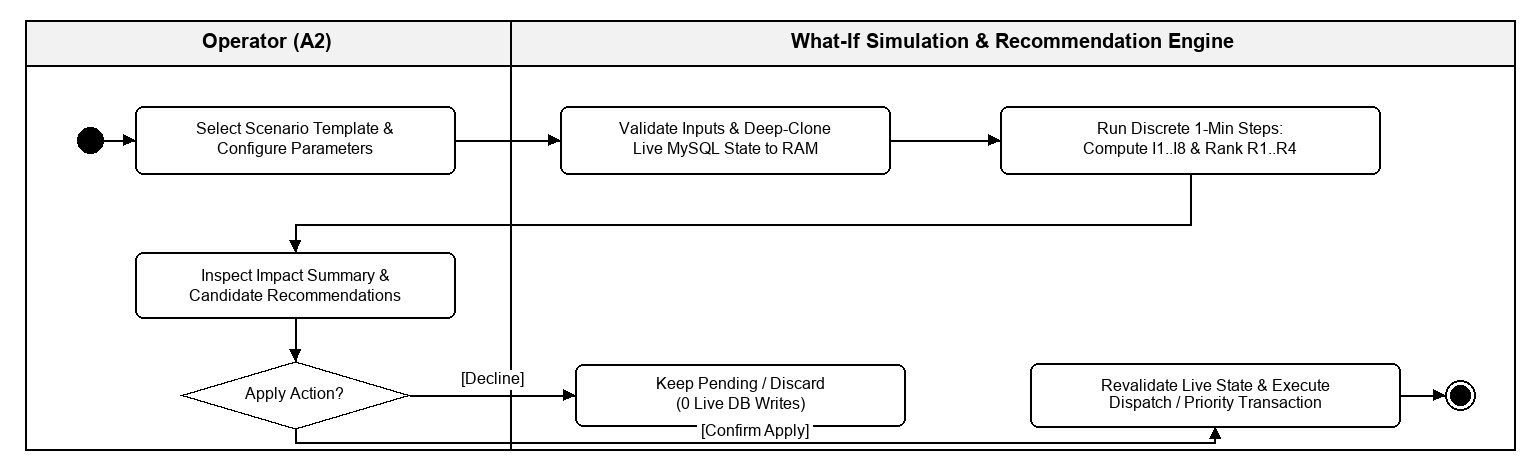
\includegraphics[width=0.90\linewidth]{graphics/diagrams/fig3_5_act_whatif.png}
  \caption{Activity Diagram --- Isolated What-If Simulation \& Live Revalidation}
  \label{fig:act-sim}
\end{figure}

\safesubsection{Sequence Diagrams}
\label{subsec:sequence-diagrams}
Four UML 2.5 Sequence Diagrams formalize chronological message ordering across actors, React UI views, Express REST Controllers, Domain Services, MySQL 8.0 InnoDB transactions, and the In-Memory Sandbox: Shared EV reservation, approval, and QR pickup (\Cref{fig:seq-reserve}); concurrent multi-charger scheduling (\Cref{fig:seq-charging}); two-phase slot-to-slot redistribution (\Cref{fig:seq-dispatch}); and What-If simulation execution (\Cref{fig:seq-sim}).

\begin{figure}[H]
  \centering
  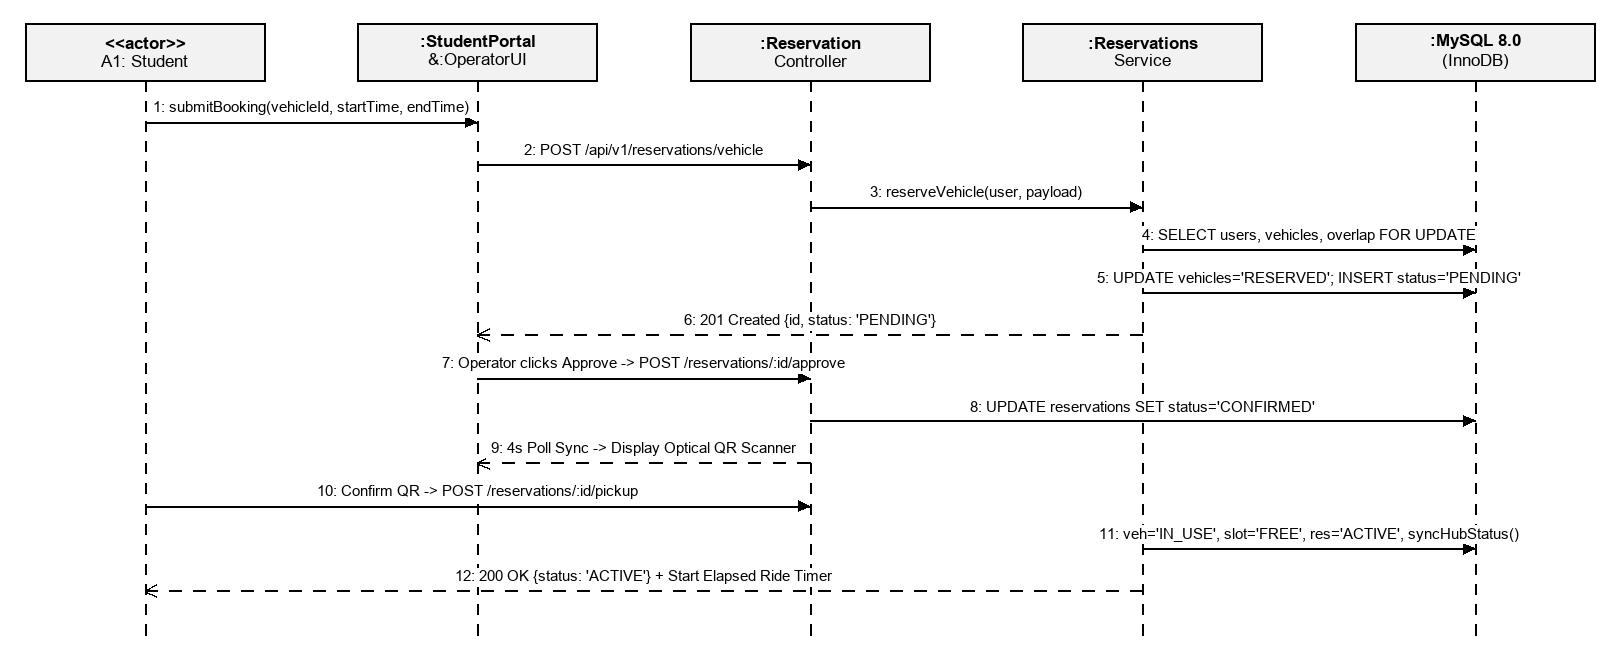
\includegraphics[width=0.92\linewidth]{graphics/diagrams/fig3_6_seq_reserve.png}
  \caption{Sequence Diagram --- Reserve Shared EV, Operator Approval \& Optical QR Pickup}
  \label{fig:seq-reserve}
\end{figure}

\begin{figure}[H]
  \centering
  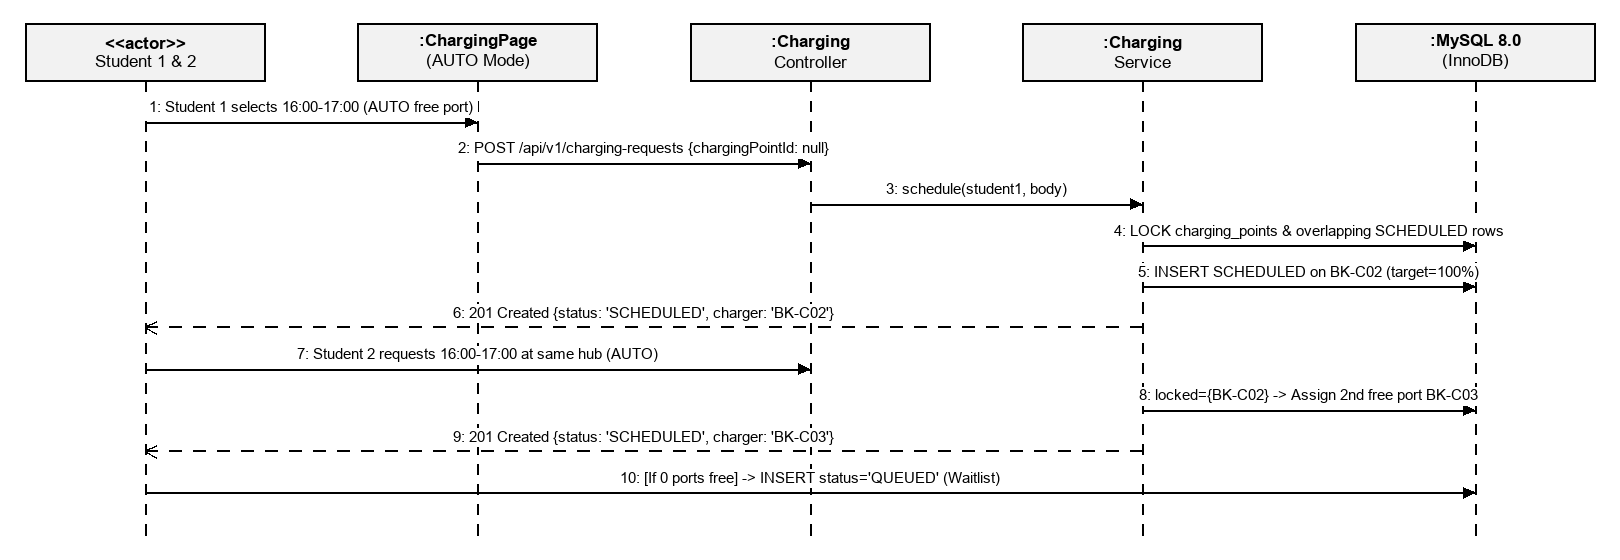
\includegraphics[width=0.92\linewidth]{graphics/diagrams/fig3_7_seq_charging.png}
  \caption{Sequence Diagram --- Concurrent Multi-Charger Scheduling \& Priority Waitlist}
  \label{fig:seq-charging}
\end{figure}

\begin{figure}[H]
  \centering
  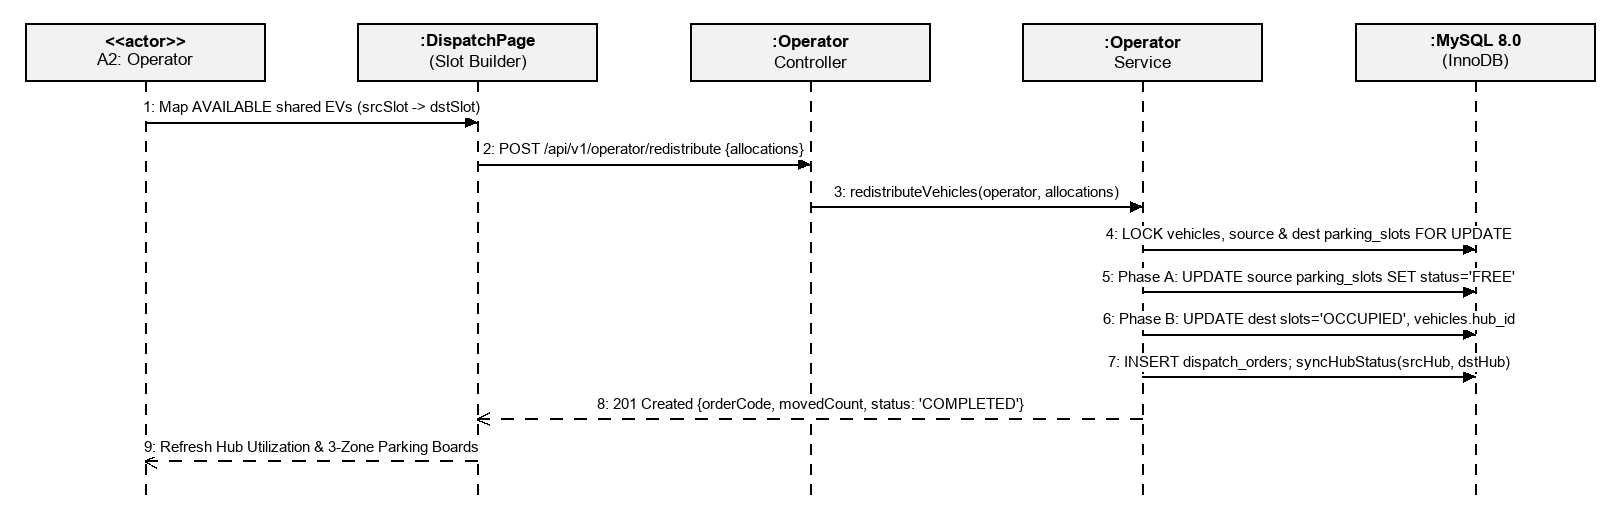
\includegraphics[width=0.92\linewidth]{graphics/diagrams/fig3_8_seq_dispatch.png}
  \caption{Sequence Diagram --- Two-Phase Slot-to-Slot Vehicle Redistribution}
  \label{fig:seq-dispatch}
\end{figure}

\begin{figure}[H]
  \centering
  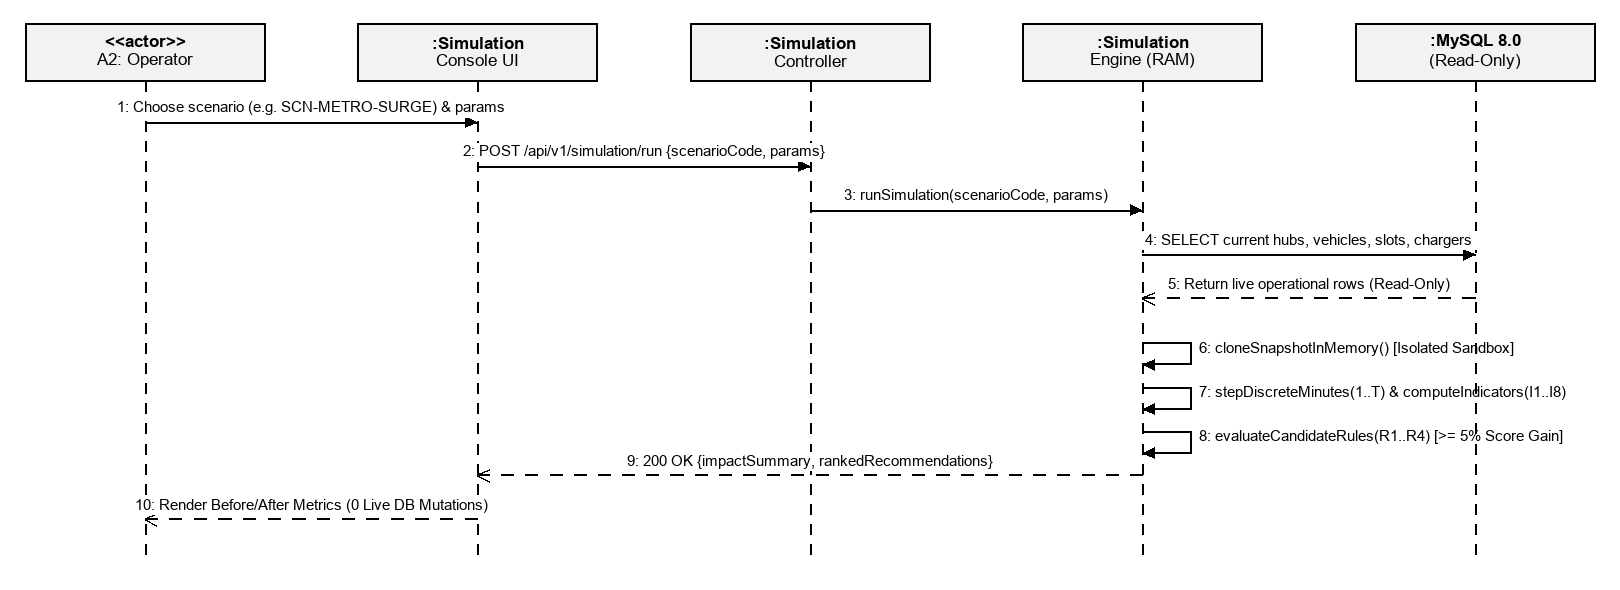
\includegraphics[width=0.92\linewidth]{graphics/diagrams/fig3_9_seq_whatif.png}
  \caption{Sequence Diagram --- Isolated What-If Scenario Execution \& Recommendation Ranking}
  \label{fig:seq-sim}
\end{figure}

\safesubsection{State Machine Diagrams}
\label{subsec:state-machines}
To prevent illegal resource mutations under concurrent operations, explicit state machines govern \texttt{Vehicle} (\Cref{fig:sm-vehicle}), the 5-stage \texttt{Reservation} lifecycle with role-safe cancellation attribution (\Cref{fig:sm-reservation}), and \texttt{ParkingSlot} / \texttt{ChargingPoint} (\Cref{fig:sm-slot-charger}).

\begin{figure}[H]
  \centering
  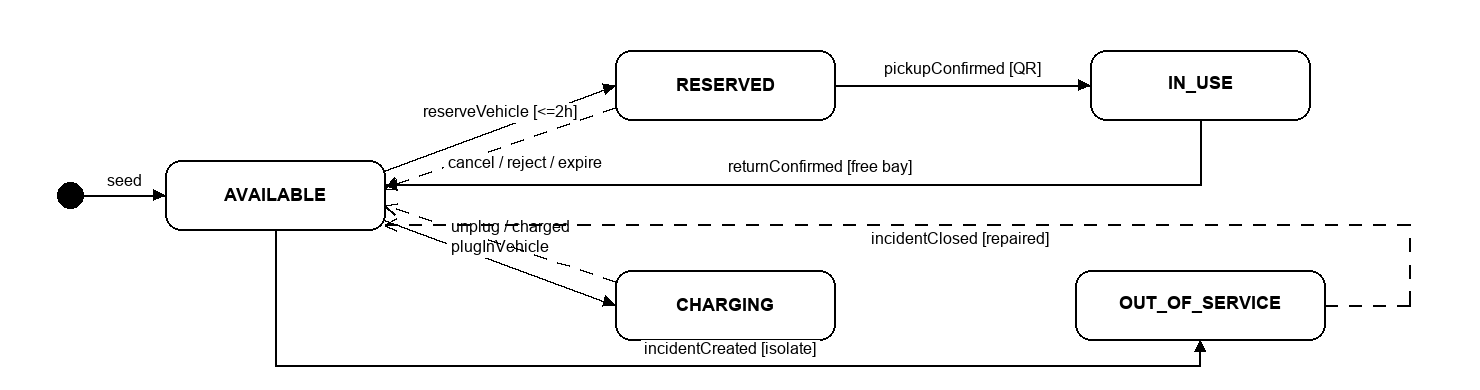
\includegraphics[width=0.90\linewidth]{graphics/diagrams/fig3_10_sm_vehicle.png}
  \caption{State Machine Diagram --- Shared Fleet \texttt{Vehicle} Lifecycle}
  \label{fig:sm-vehicle}
\end{figure}

\begin{figure}[H]
  \centering
  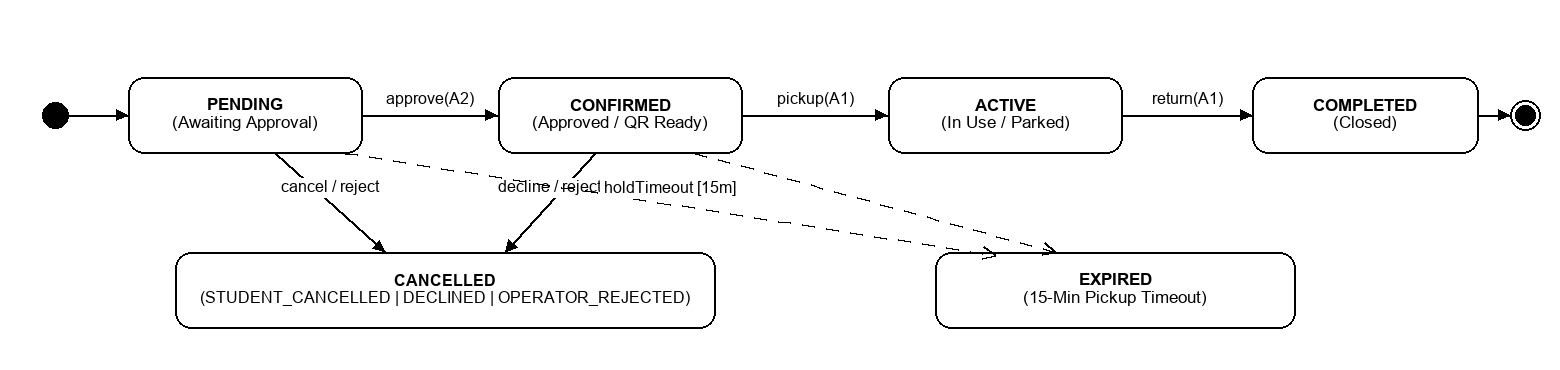
\includegraphics[width=0.92\linewidth]{graphics/diagrams/fig3_11_sm_reservation.png}
  \caption{State Machine Diagram --- 5-Stage \texttt{Reservation} Lifecycle}
  \label{fig:sm-reservation}
\end{figure}

\begin{figure}[H]
  \centering
  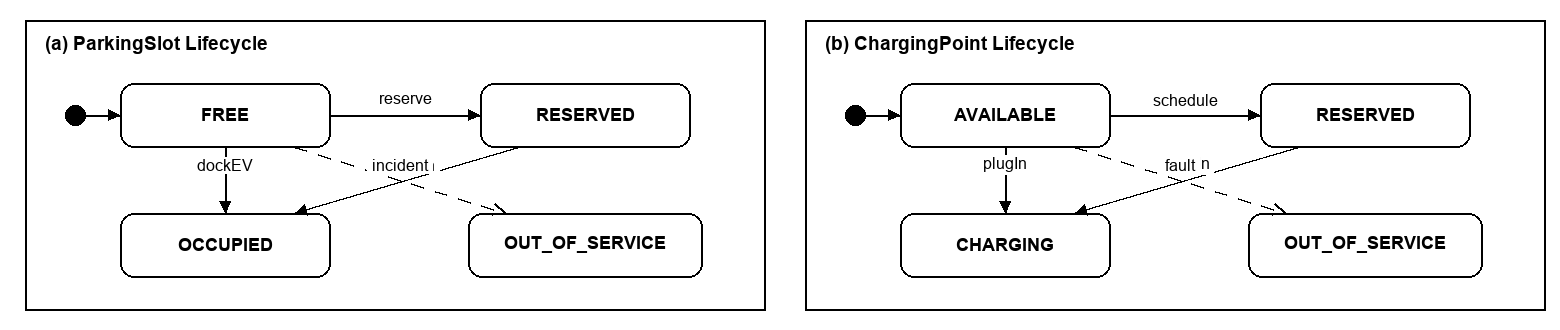
\includegraphics[width=0.92\linewidth]{graphics/diagrams/fig3_12_sm_slot_charger.png}
  \caption{State Machine Diagrams --- \texttt{ParkingSlot} and \texttt{ChargingPoint} Lifecycles}
  \label{fig:sm-slot-charger}
\end{figure}

\safesubsection{User-Interface Design}
\label{subsec:ui-design}
The V2.2 web and mobile interface separates Student (\texttt{USER}) and Staff (\texttt{OPERATOR}) workspaces behind a unified VNU-HCM header featuring Dark/Light mode switching (\Cref{fig:ui-nav}). Following the structural wireframes (\Cref{fig:wf-student,fig:wf-operator}), \Cref{fig:ui-auth,fig:ui-student-map,fig:ui-student-flows,fig:ui-operator-console,fig:ui-operator-ops,fig:ui-mobile-lan} present the delivered V2.2 application screens across authentication, interactive campus hub discovery, 5-stage reservation and \texttt{AUTO} charger scheduling, operator approval and 2-table charging control, incident isolation, slot-to-slot vehicle dispatch, isolated What-If simulation, and responsive Dark-Mode mobile operation over the campus Wi-Fi LAN (\texttt{192.168.1.7:5173}). \Cref{tab:ui-screens} summarizes all screens and feedback mechanisms.

\begin{figure}[H]
  \centering
  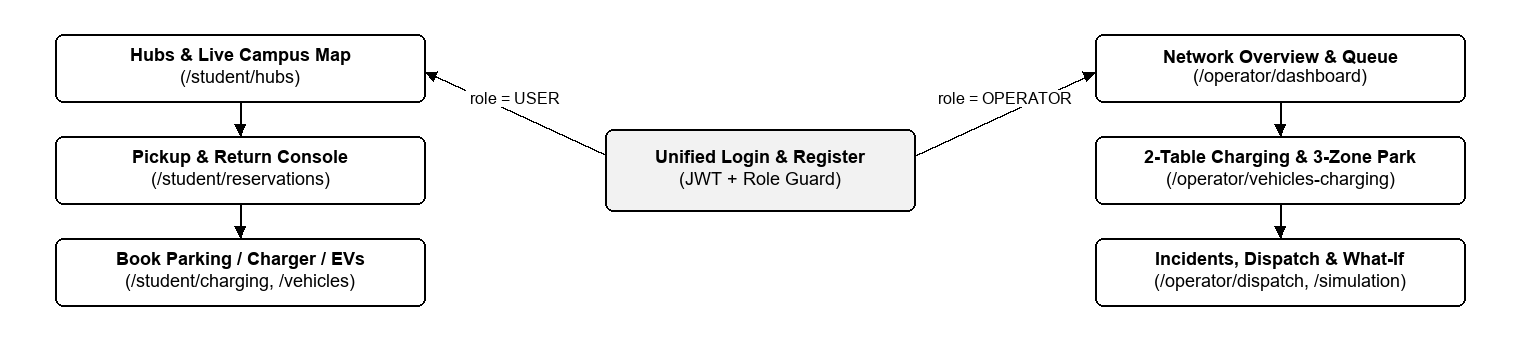
\includegraphics[width=0.90\linewidth]{graphics/diagrams/fig3_13_ui_sitemap.png}
  \caption{Role-Based Navigation Sitemap Across Student Portal and Operator Console}
  \label{fig:ui-nav}
\end{figure}

\begin{figure}[H]
  \centering
  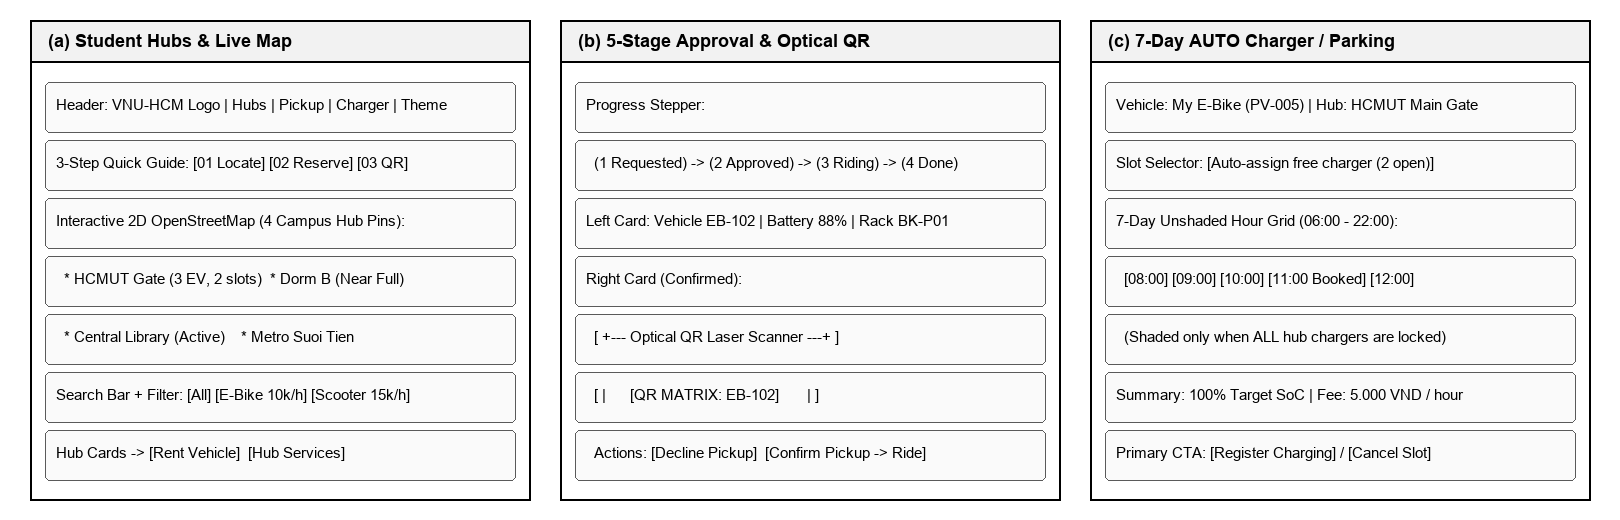
\includegraphics[width=0.94\linewidth]{graphics/diagrams/fig3_14_wf_student.png}
  \caption{Student Portal V2.2 Structural Wireframes (Live Map, QR Scanner, 7-Day \texttt{AUTO} Picker)}
  \label{fig:wf-student}
\end{figure}

\begin{figure}[H]
  \centering
  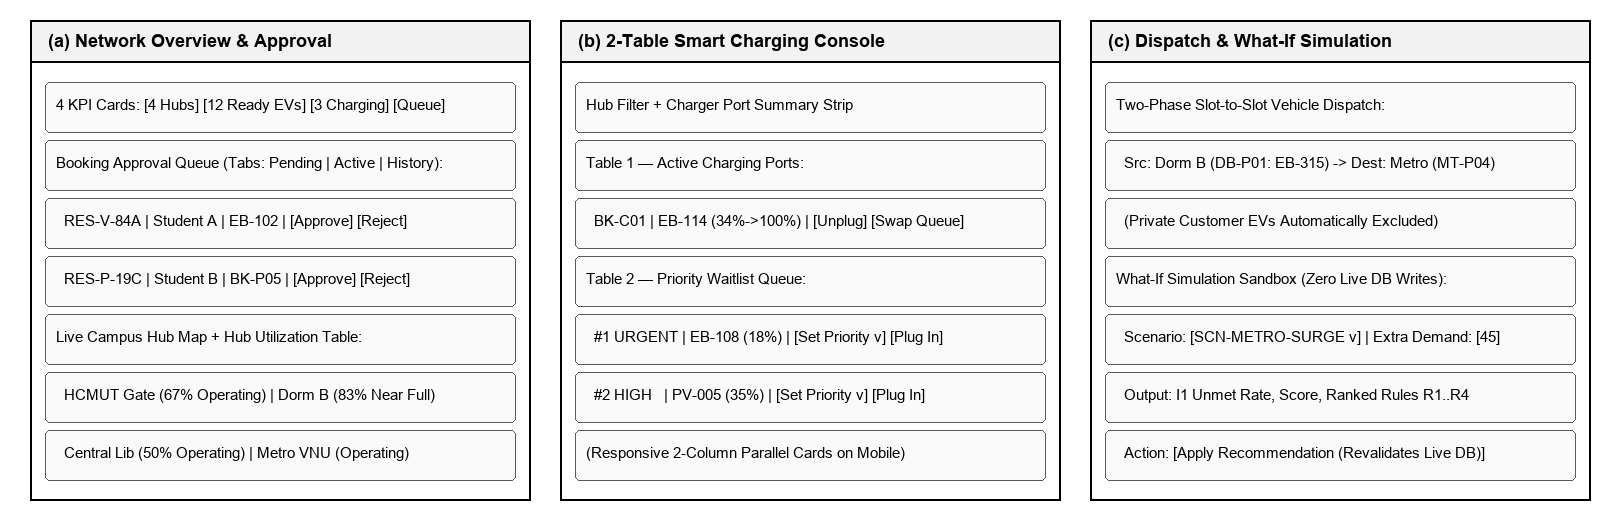
\includegraphics[width=0.94\linewidth]{graphics/diagrams/fig3_15_wf_operator.png}
  \caption{Operator Console V2.2 Structural Wireframes (Approval Queue, 2-Table Charging, What-If)}
  \label{fig:wf-operator}
\end{figure}

% --- UI PAGE PAIR A: Auth + 4-Hub Map ---
\begin{figure}[H]
  \centering
  \begin{subfigure}[t]{0.44\textwidth}
    \centering
    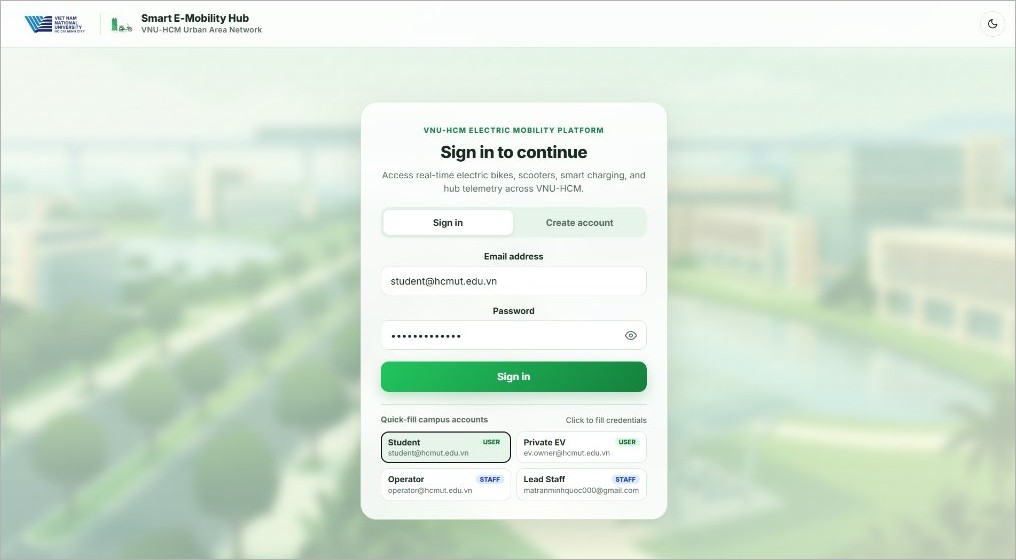
\includegraphics[width=\textwidth]{graphics/ui_v2/ui_login_student.jpg}
    \caption{Student Credential Autofill (\texttt{USER} Role)}
  \end{subfigure}\hspace{0.03\textwidth}%
  \begin{subfigure}[t]{0.44\textwidth}
    \centering
    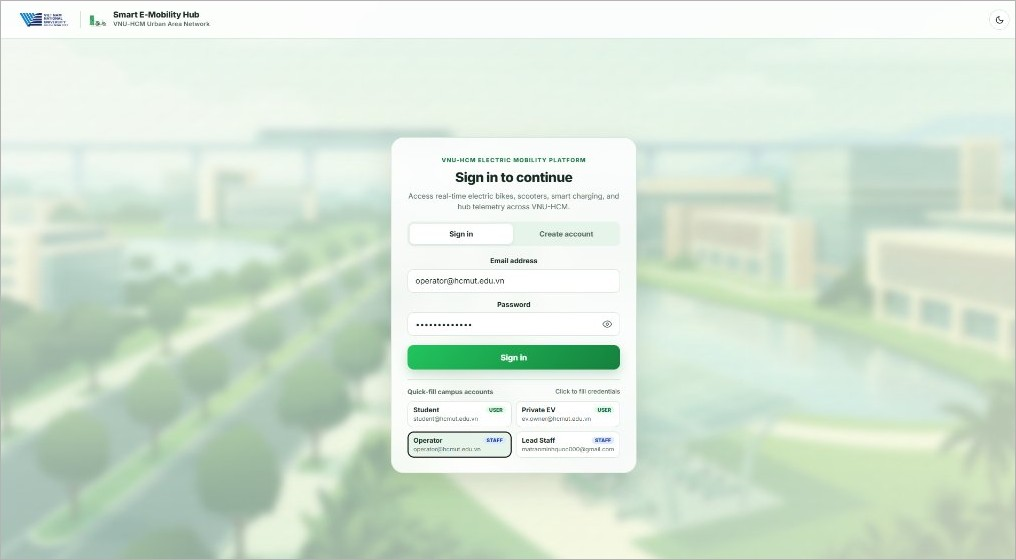
\includegraphics[width=\textwidth]{graphics/ui_v2/ui_login_operator.jpg}
    \caption{Hub Operator Credential Autofill (\texttt{OPERATOR} Role)}
  \end{subfigure}
  \caption{Delivered V2.2 Unified Authentication and Registration Interface}
  \label{fig:ui-auth}
\end{figure}

\begin{figure}[H]
  \centering
  \begin{subfigure}[t]{0.44\textwidth}
    \centering
    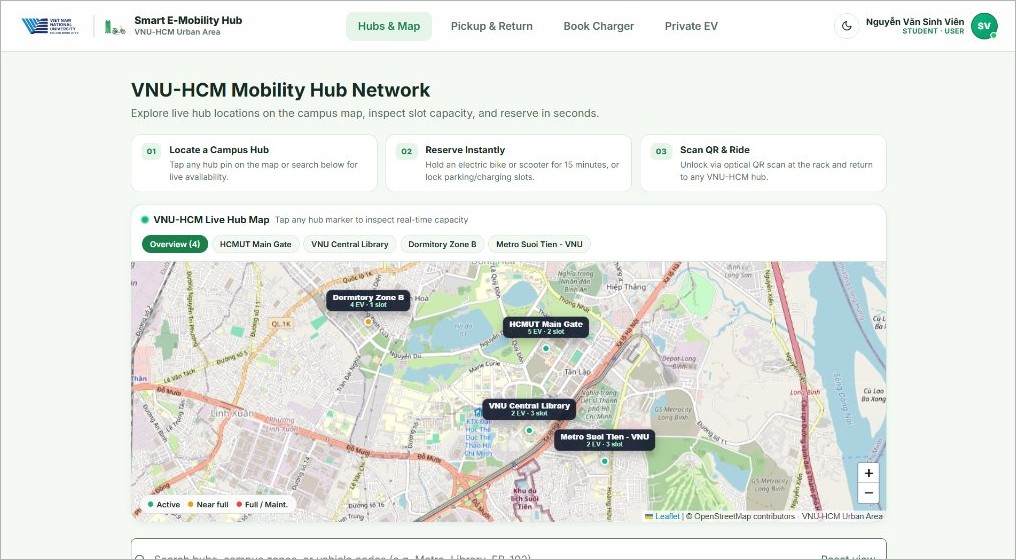
\includegraphics[width=\textwidth]{graphics/ui_v2/ui_hub_overview.jpg}
    \caption{VNU-HCM 4-Hub Network Overview \& 3-Step Guide}
  \end{subfigure}\hspace{0.03\textwidth}%
  \begin{subfigure}[t]{0.44\textwidth}
    \centering
    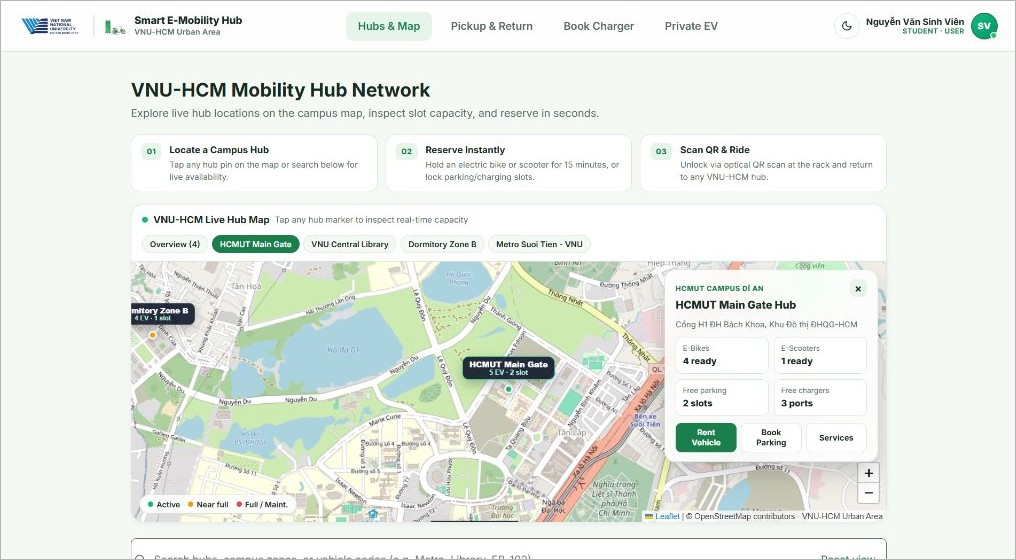
\includegraphics[width=\textwidth]{graphics/ui_v2/ui_hub_hcmut.jpg}
    \caption{HCMUT Main Gate Hub Live Capacity Card}
  \end{subfigure}\\[3pt]
  \begin{subfigure}[t]{0.44\textwidth}
    \centering
    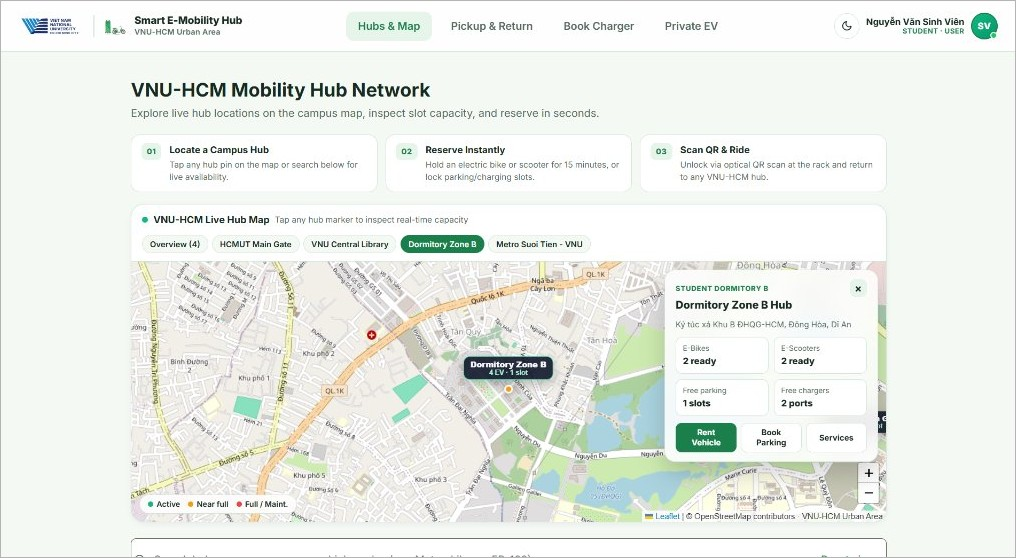
\includegraphics[width=\textwidth]{graphics/ui_v2/ui_hub_dormb.jpg}
    \caption{Dormitory Zone B Hub (\texttt{Near Full} Warning Pin)}
  \end{subfigure}\hspace{0.03\textwidth}%
  \begin{subfigure}[t]{0.44\textwidth}
    \centering
    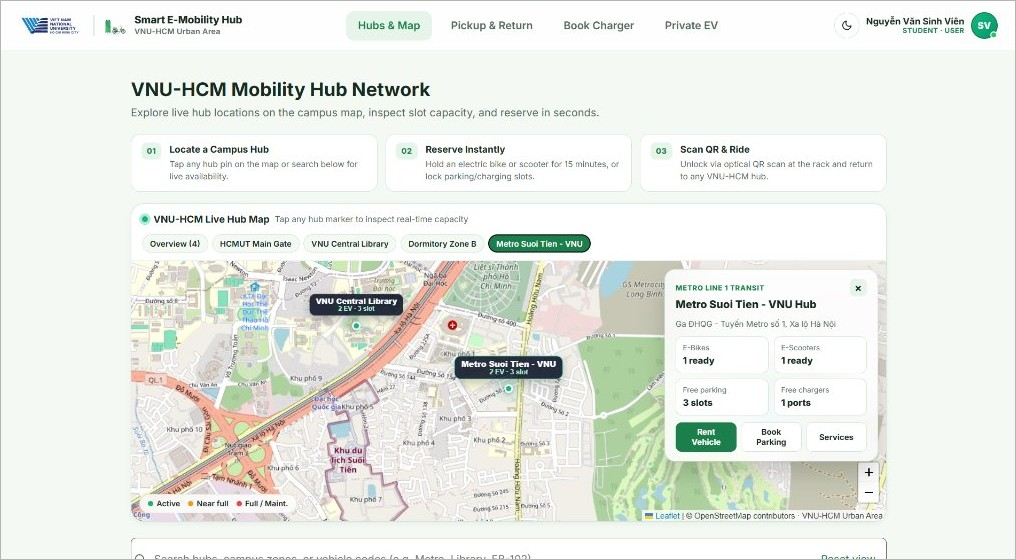
\includegraphics[width=\textwidth]{graphics/ui_v2/ui_hub_metro.jpg}
    \caption{Metro Suoi Tien -- VNU Line 1 Transit Hub}
  \end{subfigure}
  \caption{Delivered V2.2 Student Mobility Hub Network and Interactive OpenStreetMap Views (\texttt{UC01, UC02})}
  \label{fig:ui-student-map}
\end{figure}

% --- UI PAGE PAIR B: Student Flows + Operator Overview/Charging ---
\begin{figure}[H]
  \centering
  \begin{subfigure}[t]{0.44\textwidth}
    \centering
    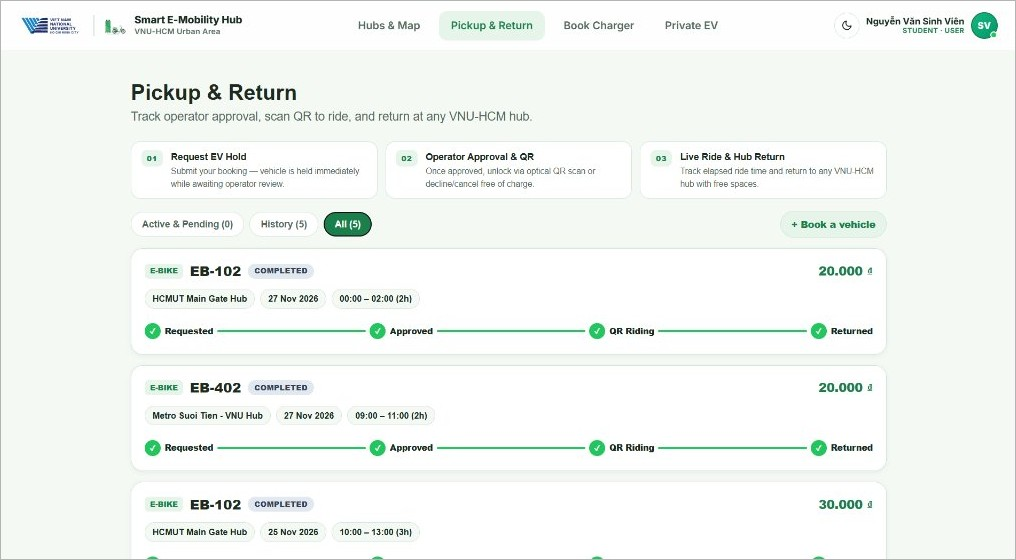
\includegraphics[width=\textwidth]{graphics/ui_v2/ui_res_completed.jpg}
    \caption{Completed Ride Stepper \& VND Tariff}
  \end{subfigure}\hspace{0.03\textwidth}%
  \begin{subfigure}[t]{0.44\textwidth}
    \centering
    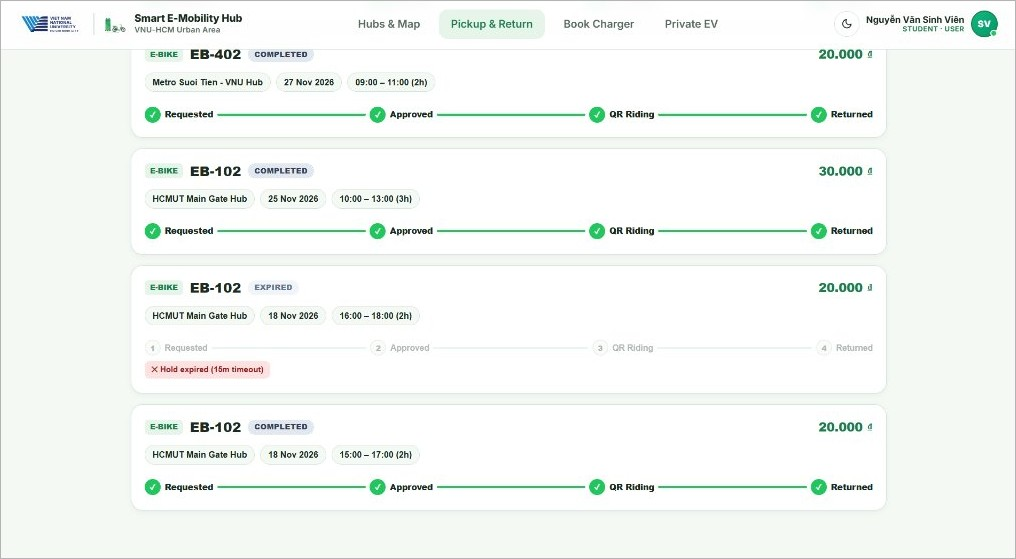
\includegraphics[width=\textwidth]{graphics/ui_v2/ui_res_expired.jpg}
    \caption{15-Minute Hold Expiration (\texttt{EXPIRED} Badge)}
  \end{subfigure}\\[3pt]
  \begin{subfigure}[t]{0.44\textwidth}
    \centering
    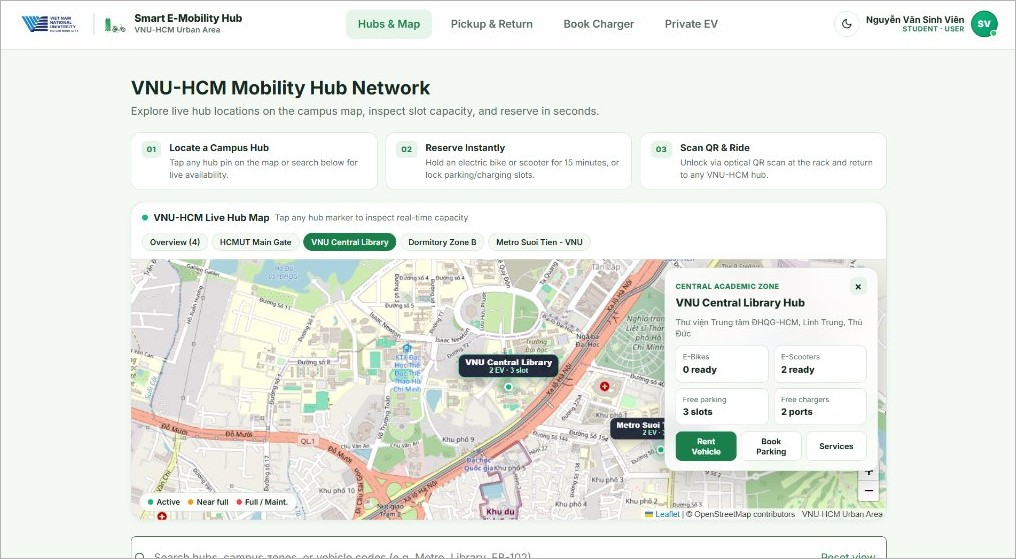
\includegraphics[width=\textwidth]{graphics/ui_v2/ui_hub_central.jpg}
    \caption{VNU Central Library Hub Selection View}
  \end{subfigure}\hspace{0.03\textwidth}%
  \begin{subfigure}[t]{0.44\textwidth}
    \centering
    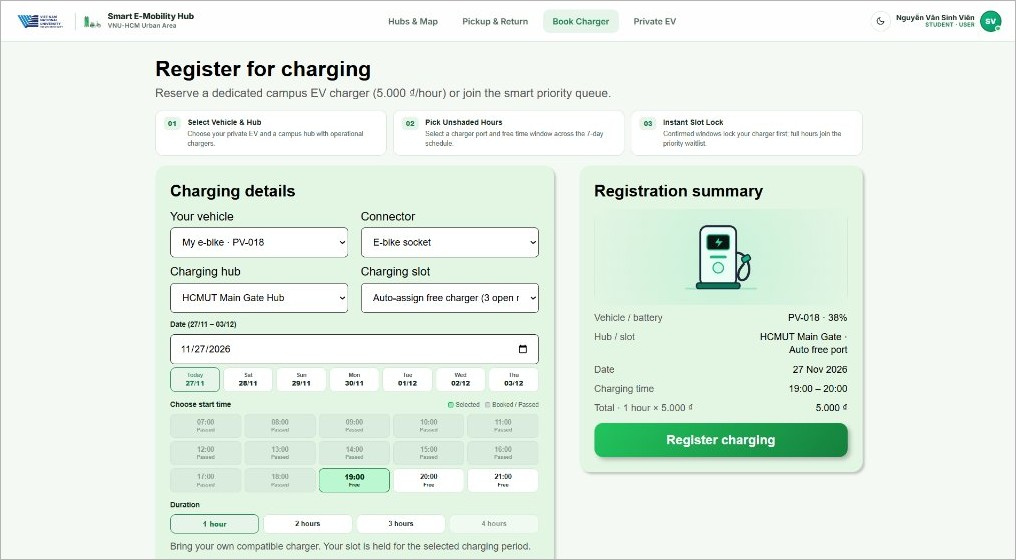
\includegraphics[width=\textwidth]{graphics/ui_v2/ui_charging_auto.jpg}
    \caption{7-Day Charger Booking with Default \texttt{AUTO} Mode}
  \end{subfigure}
  \caption{Delivered V2.2 Student Pickup/Return Lifecycle and Multi-Port \texttt{AUTO} Charger Registration (\texttt{UC04}--\texttt{UC09})}
  \label{fig:ui-student-flows}
\end{figure}

\begin{figure}[H]
  \centering
  \begin{subfigure}[t]{0.44\textwidth}
    \centering
    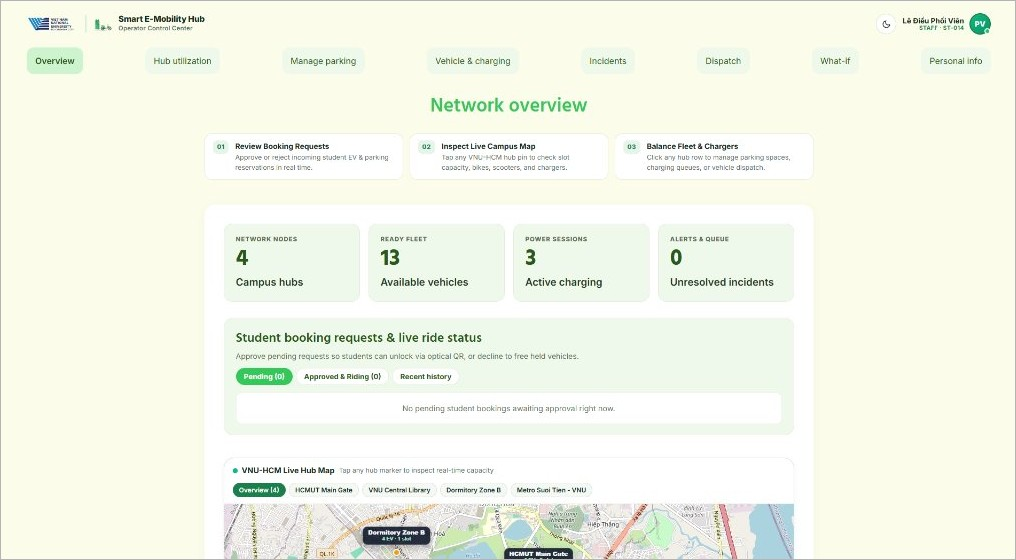
\includegraphics[width=\textwidth]{graphics/ui_v2/ui_op_overview.jpg}
    \caption{Operator Control Header \& 4 Prominent KPI Cards}
  \end{subfigure}\hspace{0.03\textwidth}%
  \begin{subfigure}[t]{0.44\textwidth}
    \centering
    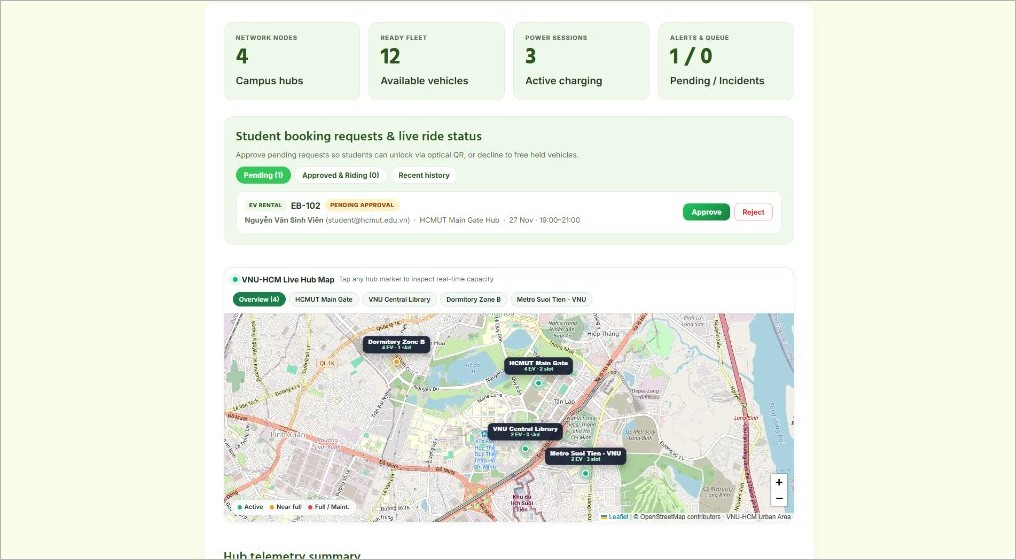
\includegraphics[width=\textwidth]{graphics/ui_v2/ui_op_approval.jpg}
    \caption{Live Booking Approval Queue (\texttt{Approve} / \texttt{Reject})}
  \end{subfigure}\\[3pt]
  \begin{subfigure}[t]{0.44\textwidth}
    \centering
    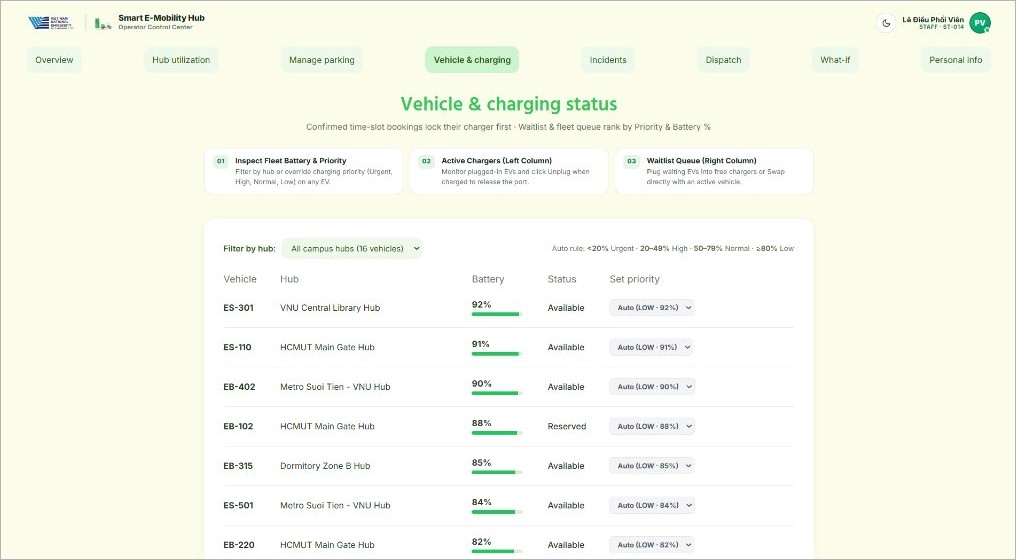
\includegraphics[width=\textwidth]{graphics/ui_v2/ui_op_fleet_soc.jpg}
    \caption{Fleet Battery Telemetry \& Priority Rules}
  \end{subfigure}\hspace{0.03\textwidth}%
  \begin{subfigure}[t]{0.44\textwidth}
    \centering
    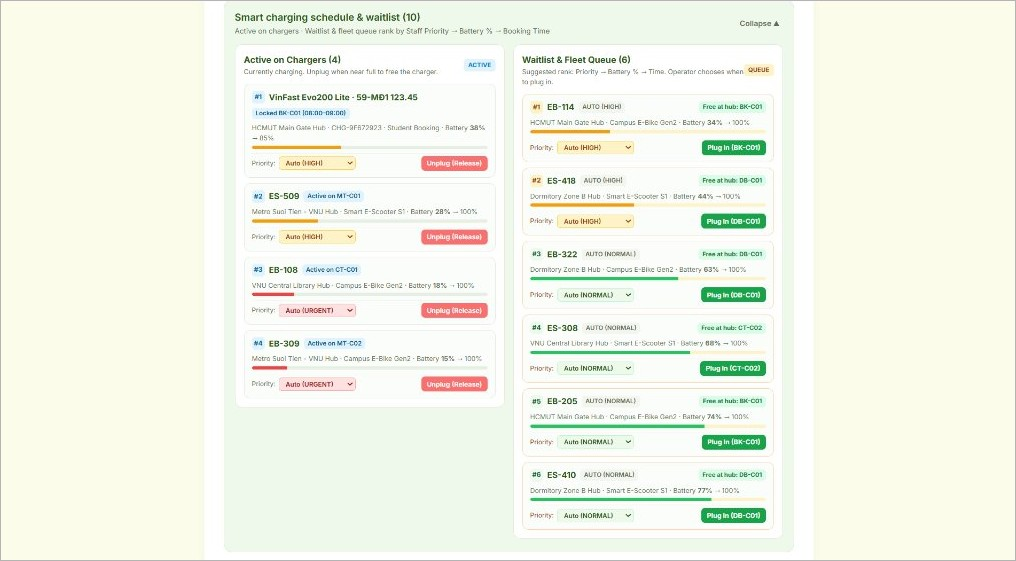
\includegraphics[width=\textwidth]{graphics/ui_v2/ui_op_charging_split.jpg}
    \caption{2-Table Split: Active Chargers vs.\ Priority Queue}
  \end{subfigure}
  \caption{Delivered V2.2 Operator Network Overview, Booking Approval, and Smart Charging Console (\texttt{UC04, UC10, UC15})}
  \label{fig:ui-operator-console}
\end{figure}

% --- UI PAGE PAIR C: Operator Ops + Mobile Dark-Mode LAN ---
\begin{figure}[H]
  \centering
  \begin{subfigure}[t]{0.44\textwidth}
    \centering
    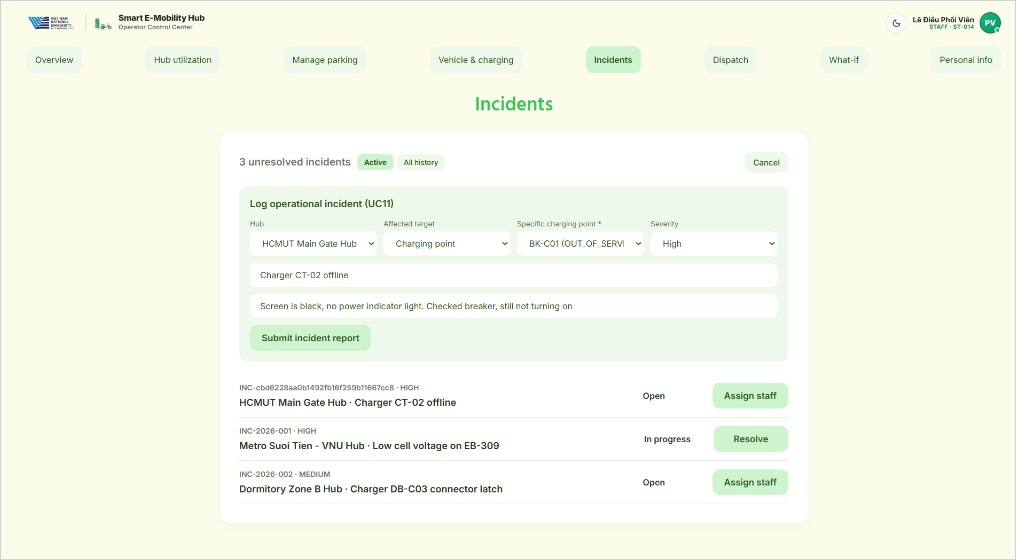
\includegraphics[width=\textwidth]{graphics/ui_v2/ui_op_incidents.jpg}
    \caption{Mandatory-Target Incident Isolation (\texttt{UC11, UC12})}
  \end{subfigure}\hspace{0.03\textwidth}%
  \begin{subfigure}[t]{0.44\textwidth}
    \centering
    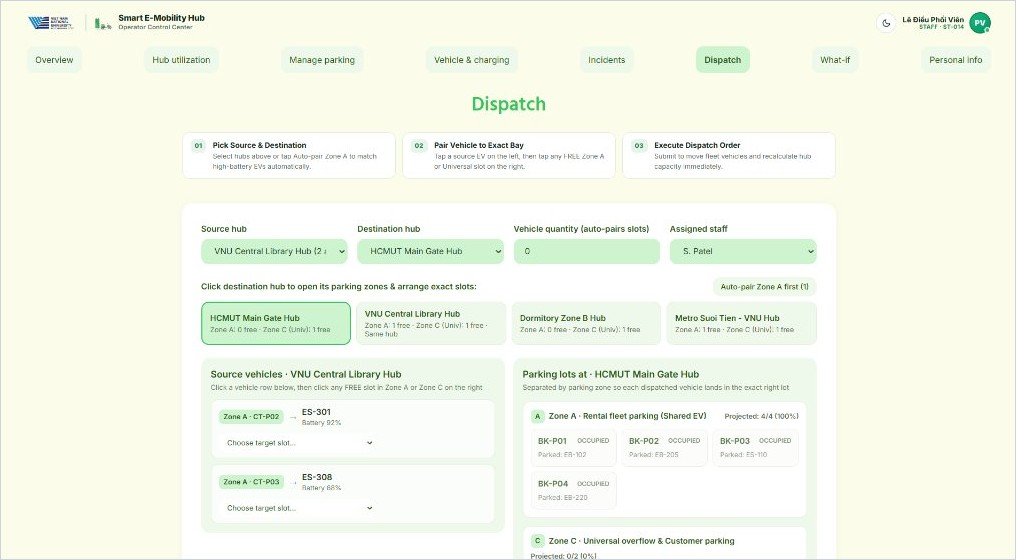
\includegraphics[width=\textwidth]{graphics/ui_v2/ui_op_dispatch.jpg}
    \caption{Slot-to-Slot Dispatch Across Zones A \& C (\texttt{UC13})}
  \end{subfigure}\\[3pt]
  \begin{subfigure}[t]{0.44\textwidth}
    \centering
    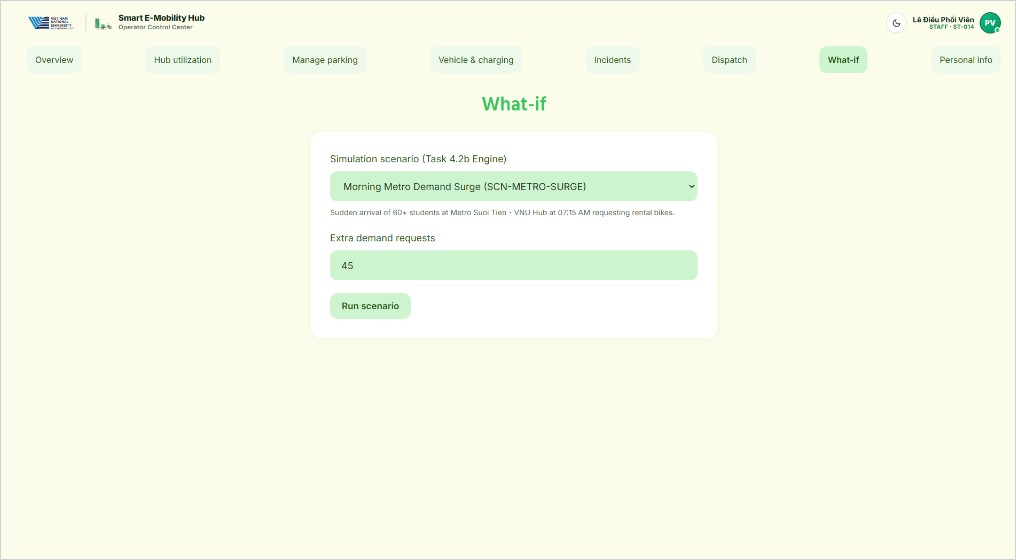
\includegraphics[width=\textwidth]{graphics/ui_v2/ui_op_whatif.jpg}
    \caption{Isolated What-If Engine (\texttt{SCN-METRO-SURGE}, \texttt{UC16})}
  \end{subfigure}\hspace{0.03\textwidth}%
  \begin{subfigure}[t]{0.44\textwidth}
    \centering
    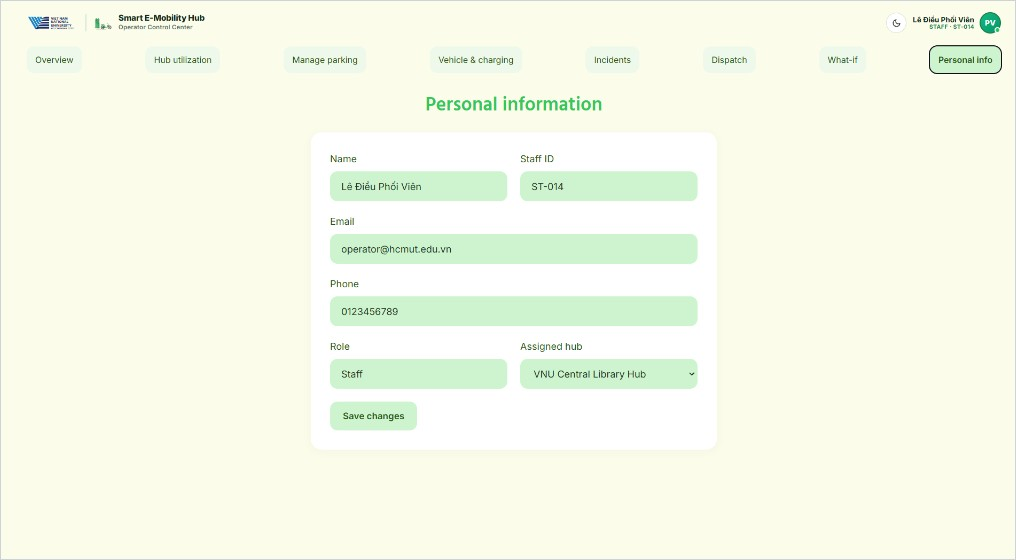
\includegraphics[width=\textwidth]{graphics/ui_v2/ui_op_profile.jpg}
    \caption{Operator Staff Profile \& Assigned Hub (\texttt{ST-014})}
  \end{subfigure}
  \caption{Delivered V2.2 Operator Incident Isolation, Slot-to-Slot Dispatch, What-If Simulation, and Staff Profile Views (\texttt{UC11}--\texttt{UC18})}
  \label{fig:ui-operator-ops}
\end{figure}

\begin{figure}[H]
  \centering
  \begin{subfigure}[t]{0.26\textwidth}
    \centering
    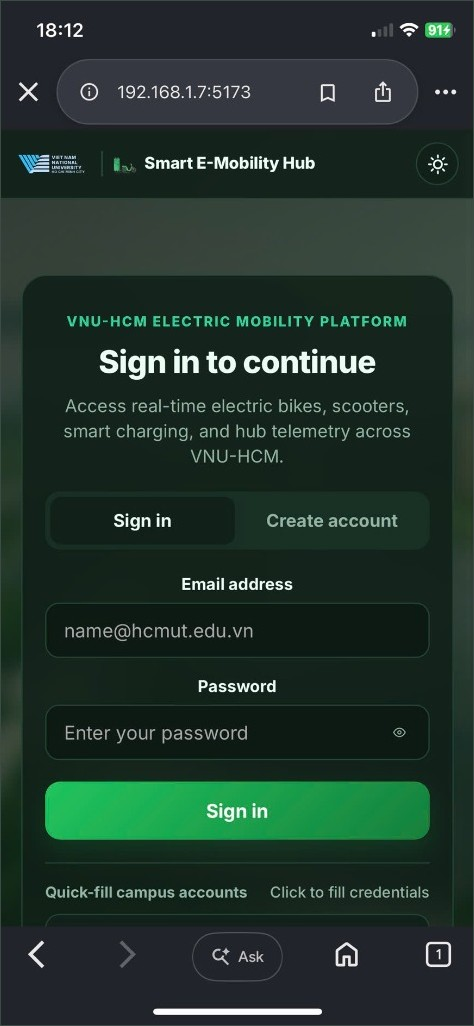
\includegraphics[width=\textwidth]{graphics/ui_v2/ui_mob_lan_url.jpg}
    \caption{Wi-Fi LAN (\texttt{192.168.1.7:5173})}
  \end{subfigure}\hspace{0.03\textwidth}%
  \begin{subfigure}[t]{0.26\textwidth}
    \centering
    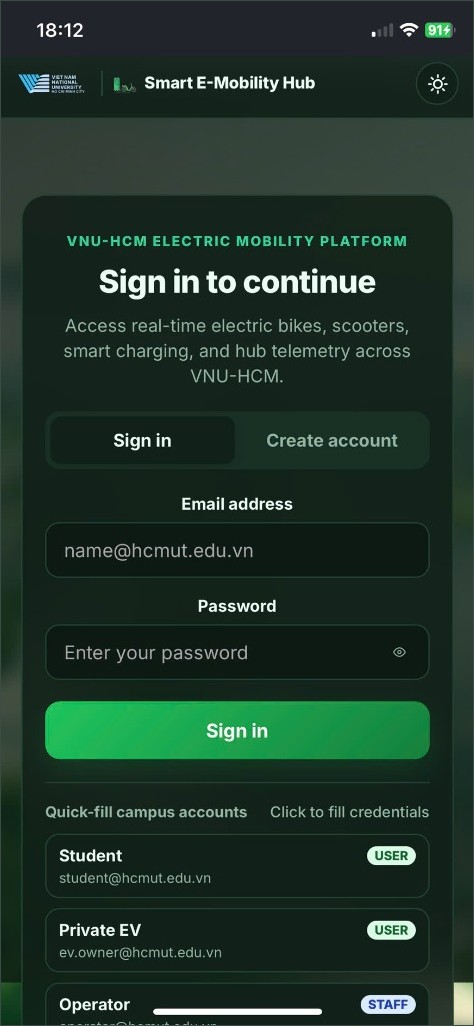
\includegraphics[width=\textwidth]{graphics/ui_v2/ui_mob_login_dark.jpg}
    \caption{Dark-Mode Auth \& Demo Chips}
  \end{subfigure}\hspace{0.03\textwidth}%
  \begin{subfigure}[t]{0.26\textwidth}
    \centering
    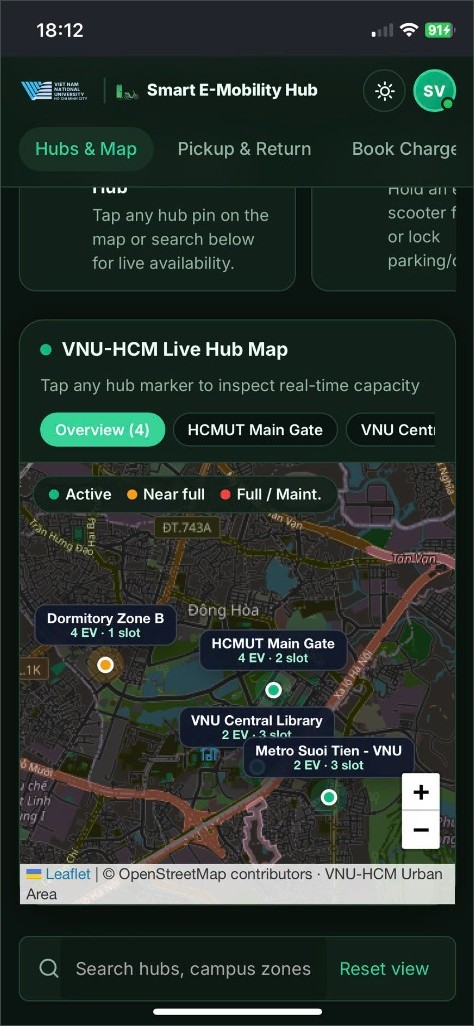
\includegraphics[width=\textwidth]{graphics/ui_v2/ui_mob_map_dark.jpg}
    \caption{Responsive Dark Live Hub Map}
  \end{subfigure}
  \caption{Delivered V2.2 Responsive Mobile Interfaces in Dark Mode over Campus Wi-Fi LAN (\texttt{192.168.1.7:5173})}
  \label{fig:ui-mobile-lan}
\end{figure}

\begin{table}[H]
  \centering
  \singlespacing\footnotesize
  \caption{Summary of Student Portal and Operator Console Screens and Feedback Mechanisms}
  \label{tab:ui-screens}
  \renewcommand{\arraystretch}{1.22}
  \begin{tabularx}{\textwidth}{|L{3.9cm}|C{1.5cm}|L{4.1cm}|Y|}
    \hline
    \rowcolor{tblHeader}
    \textbf{Screen / Route} & \textbf{Actor} & \textbf{Information Presented} & \textbf{User Actions, Feedback \& Usability Rationale} \\
    \hline
    Login \& Registration\newline(\texttt{/login}) & \texttt{A1, A2} & Email/password form, sign-up tab, VNU-HCM demo chips. & One-click demo credential autofill, password validation, automatic role routing. \\
    \hline
    Hubs \& Live Map\newline(\texttt{/student/hubs}) & \texttt{A1} & 2D OpenStreetMap pins, 3-step onboarding strip, live bike/scooter/slot counts. & Tap map pins, filter by EV type, search autocomplete; color-coded saturation badges. \\
    \hline
    Pickup \& Return\newline(\texttt{/student/\allowbreak reservations}) & \texttt{A1} & 5-stage progress stepper, EV SoC, rack code, VND fee, elapsed ride timer. & Submit hold, $4\text{ s}$ live approval sync, optical QR unlock, role-safe cancel, return hub selector. \\
    \hline
    Book Parking \& Charger\newline(\texttt{/student/\allowbreak charging}) & \texttt{A1} & 7-day hour grid, \texttt{AUTO} port/bay selector, $100\%$ target SoC, VND summary. & Hours remain selectable until \emph{all} hub ports/bays are booked, preventing false port collisions. \\
    \hline
    Network Overview\newline(\texttt{/operator/\allowbreak dashboard}) & \texttt{A2} & 4 prominent KPI cards, Booking Approval Queue, live map, utilization table. & Instant \textit{Approve} / \textit{Reject} buttons with toast confirmation and 10-second telemetry refresh. \\
    \hline
    2-Table Charging \& Parking\newline(\texttt{/operator/*}) & \texttt{A2} & Parallel Active Chargers vs.\ Priority Waitlist tables; Zones A/B/C slot cards. & \texttt{Set Priority} (\texttt{URGENT..LOW}), \texttt{Plug-in}, \texttt{Swap}, \texttt{Unplug}, and Zone C check-in/out; 2-column mobile grid. \\
    \hline
    Incidents, Dispatch \& What-If\newline(\texttt{/operator/*}) & \texttt{A2} & Open/closed incidents, slot-to-slot builder, scenario controls \& \texttt{I1..I8} metrics. & Mandatory target-unit picker, private-EV exclusion in dispatch, isolated Before/After simulation preview. \\
    \hline
    Mobile Dark-Mode LAN\newline(\texttt{192.168.1.7:\allowbreak 5173}) & \texttt{A1, A2} & Portrait single-column cards, dark-themed Leaflet tiles, touch pill navigation. & Zero horizontal overflow across $360\text{ px}$--$430\text{ px}$ viewports, Dark/Light toggle, live LAN API sync. \\
    \hline
  \end{tabularx}
\end{table}
